\documentclass[a4paper,10pt]{report}
\usepackage[utf8]{inputenc}
\usepackage[pdftex]{graphicx}
\usepackage{fancyhdr}
\usepackage{listings}
\usepackage[francais]{babel}
\usepackage{hyperref}
\usepackage{amsmath}

% Title Page
\title{IA01 : TP1}
\author{Par Camille Gerin-Roze et Thomas Perrin}



\renewcommand{\footrulewidth}{1pt}
\fancyfoot[C]{\textbf{\thepage}} 	
\fancyfoot[L]{}

\hypersetup{
	colorlinks=true,
	linkcolor=black
}

\begin{document}

\begin{titlepage}

\begin{flushright}
  
\includegraphics[scale = 0.2]{logo_utc.jpg}
\end{flushright}
\vspace*{5cm}

\newcommand{\HRule}{\rule{\linewidth}{0.5mm}} % Defines a new command for the horizontal lines, change thickness here
\center % Center everything on the page
 


%----------------------------------------------------------------------------------------
%	TITLE SECTION
%----------------------------------------------------------------------------------------

\HRule \\[0.4cm]
{ \LARGE \bfseries  IA01 : Rapport du TP1}\\[0.4cm] % Title of your document
\HRule \\[1.5cm]
 
%----------------------------------------------------------------------------------------
%	AUTHOR SECTION
%----------------------------------------------------------------------------------------
\begin{minipage}{0.4\textwidth}
\begin{flushleft} \large
\emph{Auteurs:}\\
Camille \textsc{Gerin-Roze} \newline
Thomas \textsc{Perrin} 
\end{flushleft}
\end{minipage}
~
\begin{minipage}{0.4\textwidth}

\end{minipage}\\[1.3cm]


{\large Le 2 Octobre 2015} % Date, change the \today to a set date if you want to be precise

\end{titlepage}
\tableofcontents

\chapter{Exercice 1}

  \section{Ecriture préfixée}
  
  $$4x^3 – 5x^2 + 3x + 1 $$ devient \begin{center}(+ (* 4 x x x) (* -5 x x) (* 3 x) 1 )\end{center}
  
  \section{Représentation sous forme d'arbre}
  \subsection*{Arbre généalogique}
  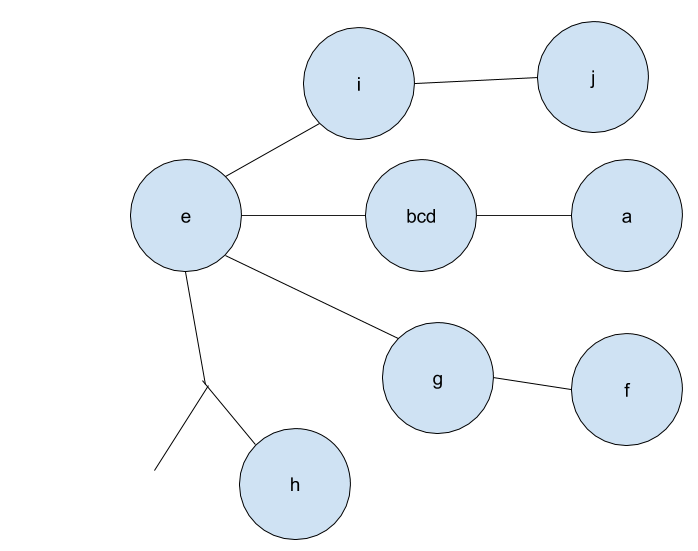
\includegraphics[scale = 0.4]{schema}\newline
  Voici la représentation sous forme d'arbre généalogique. Tous les éléments qui sont au même niveau dans la liste, sont au même niveau dans l'arbre.
  \subsection*{Arbre binaire}
  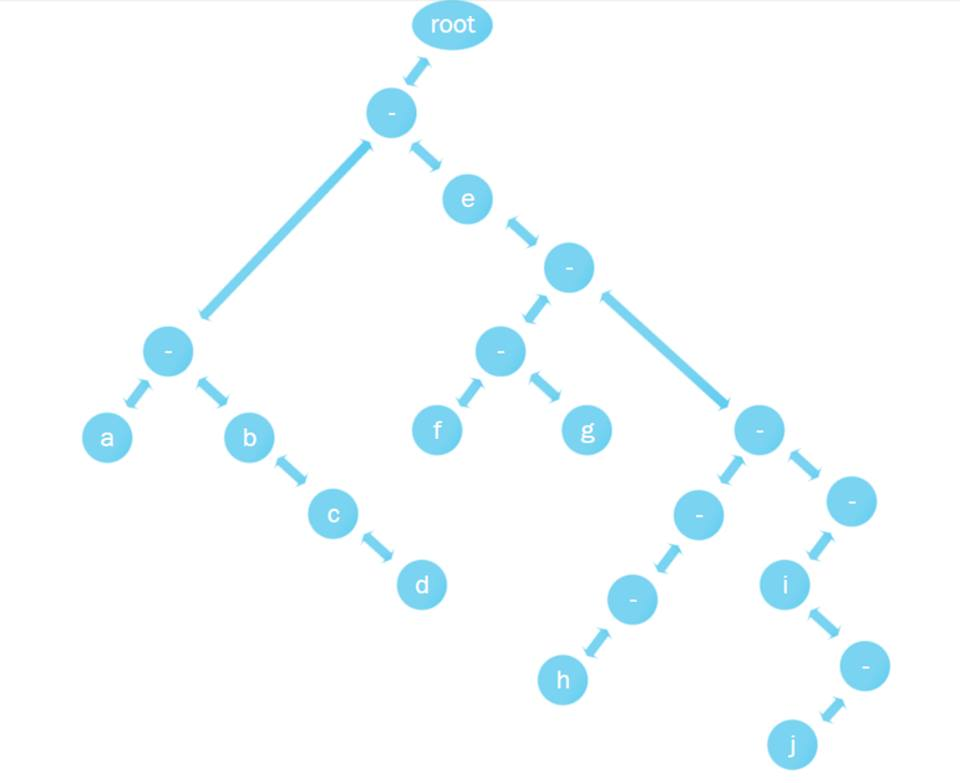
\includegraphics[scale = 0.4]{arbreBinaire}\newline
  L'arbre binaire est représenté de la façon suivante : le lien gauche est un fils, le lien de droite est un frère. Concernant le caractère " - ", il représente le début d'une sous-liste, tandis que "root" représente la racine, c'est-à-dire le début de la liste principale.

  
  \newpage
  \section{Donner les premiers N éléments}
  \subsection{Version récursive}
  \begin{lstlisting}[language=Lisp]
(defun firstn (n l)
  (if (and (> n 0) (car l)) 
  (append (list (car l)) (firstn (- n 1) (cdr l)))))
  \end{lstlisting}

  La fonction prend deux arguments :
  \begin{itemize}
   \item Le nombre d'éléments \textbf{n} à prélever dans la liste
   \item La liste \textbf{l} dans laquelle nous allons prélever les éléments
  \end{itemize}
  On prend le premier argument de la liste l, et on construit une nouvelle liste avec un appel récursif de la fonction avec \textbf{n-1} éléments, 
  jusqu'à ce que n soit égale à 0 ou que la liste soit finie ( On aurait pu également déclencher une erreur si la longueur de la liste est inférieur à n ). \newline
    \subsection{Version itérative}
  \begin{lstlisting}[language=Lisp]
    
(defun firstn-ite (n l)
  (let ((listeEntiere l))
    (setq liste ())
  (dotimes (x n liste)
    (if (not (null listeEntiere) ) (progn 
    (setq liste (append liste (list (car listeEntiere))))
    (setq listeEntiere (cdr listeEntiere))
    )))))

  \end{lstlisting}
  
  La fonction itérative se déroule différement. On crée une nouvelle liste dans laquelle on va copier les n premiers éléments. 
  On doit donc utiliser deux listes différentes. La fonction dans son format itératif utilise donc plus de mémoire. 
  
	  \subsection{Jeu de tests}
	  	\begin{lstlisting}[language=Lisp]
(firstn 3 '( 1 5))
(1 5)
(firstn 3 '( 1 5 6 4 8))
(1 5 6)
(firstn -3 '( 1 5 6 4 8))
NIL
(firstn-ite -3 '( 1 5 6 4 8))
NIL
(firstn-ite 3 '( 1 5 6 4 8))
(1 5 6)
(firstn-ite 3 '( 1 5))
(1 5)
		 \end{lstlisting}

    \newpage
    \section{Intersection de 2 listes}
    
    La méthode member ne prend pas les sous-liste en compte car elle utilise EQL et non EQUAL. On définit donc un méthode \textbf{mymember} qui utilisera EQUAL à la place de EQL :
\begin{lstlisting}[language=Lisp]
(defun myMember (x l)
  (if (not (null l))
      (if (equal x (car l)) l (myMember x (cdr l)))))
\end{lstlisting}
    
    
      \subsection{Version récursive}
	\begin{lstlisting}[language=Lisp]
(defun inter (l1 l2)
  (if (not (null (car l1)))
      (if (mymember (car l1) l2)
	 (append (list (car l1)) (inter (cdr l1) l2)) ;;; Si
	(inter (cdr l1) l2)) )) ;;; Sinon
	
	
	\end{lstlisting}

      La fonction prend en paramètre deux listes (l1 et l2). Les appels récursifs continuent jusqu'à ce que le car de la première liste (celle sur laquelle nous allons itérer).
      Si le car de l1 est un membre de la liste l2, alors on va concaténer la liste contenant le car de l1 et le résultat de l'appel récursif sur le cdr de l1 et l2. Sinon
      on fera juste l'appel récursif. \newline
      
      
      \subsection{Version itérative}
      
	\begin{lstlisting}[language=Lisp]
(defun inter-iteratif (l1 l2)
    (mapcan #'(lambda (x) (if (mymember x l2) (list x))) l1))

    
    \end{lstlisting}

      La version itérative est plus simple car en utilisant mapcan (qui renvoie une nouvelle liste) on peut tout simplement itérer sur la première liste et vérifier que chaque élément et dans la deuxième.
      Si l'élément est dans la liste, alors on retourne l'élément, sinon on retourne nil. Grâce au mapcan qui utilise \textbf{cons} pour concaténer les résultats, les nil ne seront pas membre de la liste retourner par la fonction.
      \vspace{1cm}
	  \subsection{Jeu de tests}
	   \begin{lstlisting}[language=Lisp]
(inter '(1 2 3) '())
NIL	      
(inter '(1 2 3) '(2 3))
(2 3)	   
(inter '(1 2 3 (4 5 6)) '(1 2 3 (4 5 6)))
(1 2 3 (4 5 6))
(inter-iteratif '(1 2 3) '())
NIL	      
(inter-iteratif '(1 2 3) '(2 3))
(2 3)	   
(inter-iteratif '(1 2 3 (4 5 6)) '(1 2 3 (4 5 6)))
(1 2 3 (4 5 6))
		 \end{lstlisting}

      \section{Elimination des doublons d'une liste}
      On utilisera encore une fois la fonction mymember à la place de member pour pouvoir gérer les sous-listes.
      \subsection{Version récursive}
	\begin{lstlisting}[language=Lisp]
(defun elim (l1)
(if (null (car l1)) ()
  (if (mymember (car l1) (cdr l1))
      (elim (cdr l1))
    (append (list (car l1)) (elim (cdr l1))))))
	
	
	\end{lstlisting}
      
      La fonction prend en argument une liste l1, il faut alors vérifier que cette liste ne soit pas vide. Si cette liste n'est pas vide alors on vérifie que le premier élément
      n'est pas présent dans le reste de la liste, si il est présent on va rappeller la fonction sans ajouter cet élément de manière à le supprimer. Dans le cas ou l'élément
      est absent du reste de la liste, on garde l'élément et on lui ajoute le résultat de l'appel récursif sur la suite de la liste ( cdr l1 ).
      

      \subsection{Version itérative}
	\begin{lstlisting}[language=Lisp]
(defun elim-ite (l1)
  (let ((listResult ()))
    (dolist (x l1 listResult)
      (if (and (mymember x l1) (not (mymember x listResult)))
	  (setq listResult (cons x listResult))))))
	
	\end{lstlisting}

	Pour la version itérative de la fonction, on va simplement définir une nouvelle liste contenant le résultat. Puis on va itérer sur tous les éléments de notre liste passée en 
	paramètre en ajoutant à notre listResult uniquement les éléments ne s'y trouvant pas déjà.\newline
	Cet algorithme est plus simple à réaliser mais il demande plus de mémoire car on va devoir stocker le résultat dans une autre liste.
	   \subsection{Jeu de tests}
	  \begin{lstlisting}[language=Lisp]
(elim '(1 2 3 4 5 6 6 5 4 3 2))
(1 6 5 4 3 2)
(elim '(1 2 3 4))
(1 2 3 4)
(elim '(1 2 3 4 (1 2) (1 2)))
(1 2 3 4 (1 2))
(elim-ite '(1 2 3 4 (1 2) (1 2)))
((1 2) 4 3 2 1)
(elim-ite '(1 2 3 4 5 6 6 5 4 3 2))
(6 5 4 3 2 1)
(elim-ite '(1 2 3 4))
(4 3 2 1)

		 \end{lstlisting}
		 \newpage
	\section{Compteur de feuille}
	
	   \begin{lstlisting}[language=Lisp]
(defun nbfeuilles (l1) (if (null (car l1))
	   0
	 (if (listp (car l1)) 
	    (+ (nbfeuilles (car l1)) (nbfeuilles (cdr l1))) 
	    (+ 1 (nbfeuilles (cdr l1))))))
	  \end{lstlisting}

	Ici nous avons développé seulement une version récursive de l'algorithme car la représentation d'un arbre sous forme de liste entraine forcément la formation de sous-arbres et donc l'utilisation
	de la même fonction pour les traiter, un algorithme itératif ici ne serait donc pas naturel. Si la liste est nulle, la fonction retourne 0 et ne fait pas d'appel récursif,
	si elle contient une liste, on additionera les résultats des appels récursifs sur le car et le cdr. Si l'élément n'est pas une liste, alors nous avons atteint une feuille
	donc on retourne le résultat de la fonction appliquée au cdr plus un pour la feuille que nous avons atteint.
	
	  \subsection{Jeu de tests}
	\begin{lstlisting}[language=Lisp]
(nbFeuilles '( r (( t )) y ( g h ) ( j m l ) p ))
9
(nbFeuilles '( a b c ))
3
'( a b c (d e) nil ))
5
	\end{lstlisting}\newpage
	\section{Implémentation de la méthode MONEQUAL}
	  \begin{lstlisting}[language=Lisp]
(defun monEqual (e1 e2)
  (cond 
    (( and (listp e1) (listp e2) (not (null e1)) (not (null e2)))
       (and (monEqual (car e1) (car e2)) (monEqual (cdr e1) (cdr e2))))
    ((and (atom e1) (atom e2))
                (eq e1 e2))
    ((and (null e1) (null e2))
                T)
    ('T 'nil)))
	  \end{lstlisting}

	  La différence fondamentale entre EQ et EQUAL est le fait que EQUAL va analyser le contenu des listes qu'on peut lui passer en paramètre. Nous avons donc des tests différents
	  à faire en fonction de la nature des différents arguments. Nous avons déterminer 4 cas :
	  \begin{itemize}
	   \item Si les deux éléments sont des listes non nulles, alors la fonction doit utiliser l'opérateur \textbf{AND} entre la comparaison des car des deux listes, et le résultat de l'appel récursif sur le cdr.
	   \item Si les deux éléments sont des atomes, alors on vérifie juste qu'ils sont égaux avec EQ.
	   \item Si les deux éléments sont nil, alors ils sont égaux.
	   \item Si il ne rentrent pas dans les cas précédent, cela veut dire qu'ils ne sont pas de la même nature ( nil, atome ou liste ) et donc ils sont différents.
	  \end{itemize}
	  \subsection{Jeu de tests}
	  \begin{lstlisting}[language=Lisp]
(monequal 'LUC 'LUC)
T
(monequal 'LUC 'DANIEL)
NIL
(monequal '(d p f t r) '(d p f t r))
T
(monequal (car '(do re)) (cadr '(mi do sol)))
T

		 \end{lstlisting}
	  \chapter{Exercice 2}
	  
	  
	    La finalité de cet exercice est de créer une fonction list-paire qui retourne une liste des éléments par paire de deux listes précisées en paramètre.
	  \section{Implémentation}
	  \begin{lstlisting}[language=Lisp]
-- Premiere solution : Avec le mapcar
-- Les deux arguments sont les deux listes.
(defun list-paire (x y)
               (if (and (listp x) (listp y))
                 (mapcar #'(lambda (x y) (list x y)) x y)
                 "Les deux arguments doivent etre des listes !"
                 )
)
	  \end{lstlisting}

	  L’utilisation de la fonction mapcar est le but de cette exercice c’est ainsi pourquoi cette première solution l’utilise. On utilise une fonction lambda qui sera appliquée sur chacun des éléments des listes afin de créer une sous liste à chaque itération.
	  
	    \begin{lstlisting}[language=Lisp]
-- Seconde solution : recursivite
-- Les deux arguments sont les deux listes.
(defun list-paire-récursif (x y)
  (if (not (or (null (cdr x)) (null (cdr y))))
  	(cons (list (car x) (car y)) (list-paire-récursif (cdr x)      (cdr y)))
     	(list (list (car x) (car y)))
  )
)
	  \end{lstlisting}
	  
La seconde version de cette fonction met en avant l’avantage du mapcar en comparaison de la récursivité en terme de syntaxe. La condition d’arrêt de cette fonction est lorsque la paire actuelle est la dernière en vérifiant la suivante. Le principe est la concaténation des différentes listes. \newpage
	  \section{Jeu de tests}

	  \subsection{Tests basiques}
	  \begin{lstlisting}[language=Lisp]
(list-paire '(0 2 3 11) '(6 10 20 30))
(list-paire-récursif '(0 2 3 11) '(6 10 20 30))
	  \end{lstlisting}

	  \subsection{Gestion de listes de différentes tailles}
	  \begin{lstlisting}[language=Lisp]
(list-paire '(0 2 3 11 15) '(6 10 20 30))
(list-paire-récursif '(0 2 3 11 15) '(6 10 20 30))
	  \end{lstlisting}
	  
	  \chapter{Exercice 3}
	  
	  Le but de l'exercice est de développer une fonction permettant de récupérer la valeur d'une clé dans une liste de couple (clé valeur).
	  
	  \section{Implémentation}
	  \begin{lstlisting}[language=Lisp]
(defun my-assoc (list elem)
  (setq value nil)
  (dolist (x list value)
    (if ( equal (car x) elem) (setq value (cdr x)))))
	  \end{lstlisting}

	  Nous allons donc parcourir la liste grâce à la méthode \textbf{dolist} et on remplira la valeur de retour \textbf{value} si la clé du couple est celle passée en paramètre de la fonction.
	  
	  
	  \section{Jeu de tests}
	  
	  \begin{lstlisting}[language=lisp]
(setq base '((a 1) (b 2) (c 3) (abc (1 2 3)) (abab ((1 2) (1 2)))))
(my-assoc base 'a)
1
(my-assoc base 'b)
2
(my-assoc base 'c)
3
(my-assoc base 'abab)
((1 2) (1 2))
(my-assoc base 'abc)
(1 2 3)
(my-assoc base 'notHere)
NIL
	  \end{lstlisting}
Pendant les tests, on voit que la valeur retournée est la bonne même si celle-ci est une liste. Dans le cas où la clé n'existe pas, la valeur NIL sera retournée.
	  
	  
	  \chapter{Exercice 4} 
	  
	  Dans ce dernier exercice, on utilisera la base de données suivante définit dans l’énoncé :
	  \begin{lstlisting}[language=Lisp]
(setq BaseTest '((" Le Dernier Jour d'un condamne " Hugo 1829 50000)
(" Notre-Dame de Paris " Hugo 1831 3000000)
(" Les Miserables " Hugo 1862 2000000)
("Le Horla " Maupassant 1887 2000000)
(" Contes de la becasse " Maupassant 1883 500000)
("Germinal " Zola 1885 3000000)
))
	  \end{lstlisting}
	  
	  \section{Fonctions de service}
	  
	  \begin{lstlisting}[language=Lisp]
(defun auteur (ouvrage)
  (cadr ouvrage))

(defun titre (ouvrage)
  (car ouvrage))

(defun annee (ouvrage)
  (caddr ouvrage))

(defun nombre (ouvrage)
  (cadddr ouvrage))
	  \end{lstlisting}
	  
	  Ces différentes fonctions permettent de récupérer une information précise d’un ouvrage. Elles vont être réutilisées dans les fonctions suivantes.
	  \newpage
\section{Afficher tous les ouvrages}	  
\begin{lstlisting}[language=Lisp]	  
(defun affichAllOuvrage (base)
  (mapcar #'(lambda (l) (titre l)) base))
\end{lstlisting}
L’affichage des ouvrages se fait par une simple itération via un mapcar, en utilisant une fonction de base.
\section{Afficher tous les ouvrages de Hugo}	  
\begin{lstlisting}[language=Lisp]
(defun affichAllOuvrageOfHugo (base)
  (remove nil 
  (mapcar #'(lambda (l) 
  (if (EQ (auteur l) 'Hugo) (titre l) ())) base)))
\end{lstlisting}
L’affichage des ouvrages spécifique à Victor Hugo se filtre grâce à la fonction if et à la fonction auteur réalisée précédemment. On retire les NIL via la fonction remove.
\section{Afficher tous les ouvrages d'un auteur}	  
\begin{lstlisting}[language=Lisp]
(defun affichAllOuvrageOfAutor (base autor)
  (remove nil 
  (mapcar #'(lambda (l) 
  (if (EQ (auteur l) autor) (titre l) ())) base)))
\end{lstlisting}
Le filtrage par un auteur en paramètre se réalise de la même manière en utilisant un argument supplémentaire au lieu d’utiliser un mot brut.
\section{Afficher le premier ouvrage d'une année}	  

\begin{lstlisting}[language=Lisp]
(defun affichFirstOuvrageOf (base year)
  (dolist (l base) (if (EQ (annee l) year) (return (titre l)))))
\end{lstlisting}
Dans cette fonction, nous utilisons un dolist afin de pouvoir s’arrêter dès que la condition est satisfaite, à l’aide encore une fois d’une fonction de service.
\section{Afficher les ouvrages vendue à plus de 100k exemplaires}	  

\begin{lstlisting}[language=Lisp]
(defun affichOuvrageWithMore100k (base)
  (remove nil 
  (mapcar #'(lambda (l) 
  (if (>= (nombre l) 100000) (titre l) ())) base)))
\end{lstlisting}
Retour à l’utilisation du mapcar puisqu’on itère sur toute la liste. Nous vérifions le nombre d’exemplaires grâce à une fonction de service.\newpage
\section{Afficher la moyenne du nombre de ventes de l'ouvrage d'un auteur}	  
\begin{lstlisting}[language=Lisp]
defun moyenne (base aut)
  (let ((nbExemplaire 0.0)(sum 0.0))
   (/ (dolist (livre base sum)
   (if (equal aut (auteur livre))
     (progn 
     (setq nbExemplaire (+ nbExemplaire 1))
     (setq sum (+ sum (cadddr livre)))))
   ) nbExemplaire )))
\end{lstlisting}
Enfin, la fonction de la moyenne est réalisée à l’aide d’un dolist et de variable. Le let au départ permet de définir les variables sum et nbExemplaire afin de retenir le nombre d’exemplaires et d’ouvrages pour finalement réaliser à la fin la division. La variables sum retournée à la fin sera divisée par le nbExemplaire.

	  
	  
	  
	  
	  
	  
	  
	  
	  
	  
	  
\end{document}          
